\documentclass[journal]{IEEEtran}
\usepackage[T1]{fontenc}
\usepackage{amsmath,amssymb}
\usepackage{graphicx}
\usepackage{booktabs}
\usepackage{multirow}
\usepackage{array}
\usepackage{xcolor}
\usepackage{tikz}
\usetikzlibrary{arrows.meta,positioning}
\usepackage[hidelinks]{hyperref}
\usepackage{cite}
\graphicspath{{../../figures/}}
\newcommand{\ms}{MRR@10}
\newcommand{\nd}{nDCG@10}
\newcommand{\fl}{$^{\dagger}$}
\newcommand{\m}{$-$}
\newcommand{\p}{$+$}

\begin{document}

\title{Decision Models as Starting Points for\\Cross-Encoder Rerankers: A Preregistered Study}

\author{Nikhil~Y~N, Mohamed~Qurrain~Shayeeb, Prithvi~K~M, and~Praneel~S%
\thanks{The authors are with the Department of Computer Science and Engineering, Ramaiah Institute of Technology, Bengaluru, India (e-mail: nikhilylkn@gmail.com; qsirius12@gmail.com; prithvikiranm791@gmail.com; praneelsindhole2005@gmail.com).}%
\thanks{Code, configuration, run logs, per-query scores and the preregistration tag: \url{https://github.com/nikhil-yn-aix/Arbiter}.}}

\markboth{Decision Models as Starting Points for Cross-Encoder Rerankers}{Y N \MakeLowercase{\textit{et al.}}}

\maketitle

\begin{abstract}
A cross-encoder reranker reorders search results by reading the query and each candidate passage together. It is trained by fine-tuning a pretrained text encoder. Several public ``decision models'', encoders fine-tuned to answer yes/no and multiple-choice questions about a passage, share one such encoder, ModernBERT-large. We ask whether starting reranker training from one of them beats starting from the plain encoder. We fine-tune eight starting points with one recipe on 250 to 16{,}000 MS MARCO training queries: the plain encoder, five decision checkpoints, a natural-language-inference (NLI) checkpoint and a randomly perturbed copy of the encoder. Each starting point gets its own learning-rate search, and the smaller budgets use multiple seeds. The analysis was frozen in a git tag before the confirmatory runs, and test scores stayed sealed until all training had ended. The preregistered result is inconclusive. At 1{,}000 queries the decision checkpoints average $+0.025$ \ms{} over the plain encoder (95\% CI $-0.052$ to $+0.101$). Most of this uncertainty comes from five of the 59 analysed runs whose training collapsed. All five started from a non-base checkpoint and used a learning rate above the plain encoder's. Exploratory analyses decided after unsealing set these runs aside. They give a head start of $+0.03$ to $+0.05$ \ms{} at 1{,}000 queries, depending on how the plain encoder's own weakest seed is treated, and no difference at 16{,}000. The head start is not specific to decision training. The NLI checkpoint gives more, and the random perturbation, when it trains, gives some. Before any fine-tuning, a frozen-feature probe of each starting point tracks its fine-tuned gain (Spearman $\rho=0.90$ over the eight starting points). Code, configurations and per-query scores are public.
\end{abstract}

\begin{IEEEkeywords}
Information retrieval, reranking, cross-encoders, transfer learning, intermediate-task training, preregistration, reproducibility.
\end{IEEEkeywords}

\section{Introduction}

\IEEEPARstart{A}{} cross-encoder reranker reads a query and a candidate passage together and outputs one number: how relevant the passage is~\cite{nogueira2019passage,lin2021survey}. Training one is simple. Start from a pretrained text encoder, show it queries with one relevant passage and a few plausible but wrong ones, and teach it to put the relevant one first~\cite{gao2021rethink}. One choice in this recipe is easy to overlook: \emph{which checkpoint do you start from?}

That choice has recently become a real one. A family of public checkpoints called \emph{decision models} has appeared~\cite{rastogi2026smallheads,dinzinger2026systemone}. A decision model is a text encoder fine-tuned to answer typed questions about a passage, such as yes/no or ``which of these options'', in one forward pass. Five of them are built on the same encoder, ModernBERT-large~\cite{warner2024modernbert}, and load into it without any change. Anyone who would start a reranker from ModernBERT-large can just as easily start from one of these.

Is that a good idea? There is a plausible case for yes. Deciding whether a passage answers a question is close to judging relevance, and training on a related task first, known as intermediate-task training, often helps a later one~\cite{phang2018stilts,pruksachatkun2020intermediate,vu2020transferability,garg2020tanda}. There is also a plausible case for no. Decision models used directly as rerankers lose to dedicated rerankers~\cite{dinzinger2026systemone,li2026replace}, and with little ranking data, extra pre-training can even hurt~\cite{zhang2020littlebit}. Those studies use decision models as finished rerankers. To our knowledge, none tests whether a decision checkpoint is a better \emph{starting point} for training one.

We test this with a design meant to avoid common pitfalls in comparing checkpoints. All eight starting points, which we call \emph{arms}, share one architecture and tokenizer, so only the weights differ. Every arm is fine-tuned with the same data, loss and schedule. We vary the amount of training data 64-fold, because a head start often matters only when data is scarce. Two controls separate decision training from cheaper explanations. The first is an NLI checkpoint, standing for generic supervised training. The second is a random perturbation of the encoder as large as a decision model's change, standing for ``any change to the weights''. Each arm gets its own learning-rate search on a development set. We froze the configuration and analysis code in a dated git tag before the confirmatory runs, and test scores stayed sealed until every run had finished.

Our findings, in order of confidence:
\begin{enumerate}
\item \textbf{The preregistered answer is ``inconclusive''} (Section~\ref{sec:primary}). Averaged over the five decision checkpoints, the difference from the plain encoder is $+0.025$ \ms{} at 1{,}000 training queries and $-0.060$ at 16{,}000, with 95\% intervals wider than 0.15. These data cannot rule out a gain, a loss or no difference.
\item \textbf{The uncertainty comes from collapsed runs} (Section~\ref{sec:collapse}). In five runs the training loss ended close to the level of random guessing. All five started from a non-base checkpoint and ran at a learning rate above the plain encoder's. Because the plain encoder never trained at those rates, we cannot tell whether the checkpoints or the rates are to blame.
\item \textbf{Without the collapses, a small head start that fades} (Section~\ref{sec:excl}, exploratory). Decision checkpoints lead by $+0.03$ to $+0.05$ \ms{} at 1{,}000 queries, depending on how the plain encoder's weakest seed is treated. They are equivalent to the plain encoder at 16{,}000.
\item \textbf{Most of the head start is not specific to decisions} (Section~\ref{sec:specific}). The NLI checkpoint beats the decision checkpoints in every analysis. When the random perturbation trains normally (exploratory), it recovers about two-thirds of the decision head start. How well a frozen checkpoint already ranks tracks its fine-tuned gain across all eight arms.
\end{enumerate}

\section{Background and Related Work}

\textbf{Cross-encoder rerankers.} BERT-style encoders fine-tuned on MS MARCO~\cite{nguyen2016msmarco} are the standard second-stage ranker~\cite{nogueira2019passage,nogueira2020monot5,lin2021survey}. They are trained on hard negatives from BM25, a classic keyword-matching ranker~\cite{robertson2009bm25}. A softmax over one positive and several such negatives (a ``listwise'' or localized-contrastive loss) works better than scoring passages one at a time~\cite{gao2021rethink}. Effectiveness grows smoothly with model and data size~\cite{seetharaman2026scaling}. A separate earlier fine-tuning stage brings no clear gain over one well-tuned contrastive stage~\cite{pezzuti2025multistage}. Transfer and pseudo-labelling help BERT rankers mainly when target data is small~\cite{mokrii2021transfer}, and with very little data, fine-tuning can end up worse than an unsupervised ranker~\cite{zhang2020littlebit}. We study the input to this pipeline: what the encoder knows \emph{before} reranker training starts.

\textbf{Decision models.} These are encoders that answer typed questions about text (yes/no, choice, score) in one forward pass, usually trained for calibrated probabilities. Controlled comparisons find that the design of the small output head matters little~\cite{rastogi2026smallheads}. Used directly as rerankers, decision models lose to rerankers fine-tuned from the same backbone~\cite{dinzinger2026systemone}. Replacing a reranker with one in a retrieval pipeline trades quality against speed and memory~\cite{li2026replace}. These studies use decision models as \emph{finished} rankers. We use them as \emph{starting points}.

\textbf{Intermediate-task transfer.} Fine-tuning on a related labelled task before the target task can help, especially when target data is scarce~\cite{phang2018stilts}. NLI and question answering are among the most reliably useful intermediate tasks~\cite{pruksachatkun2020intermediate,vu2020transferability}, and transfer through answer selection helps related ranking-style tasks~\cite{garg2020tanda}. Simple frozen-feature probes can predict which intermediate task will help~\cite{poth2021pretrain,kornblith2019transfer}. Our NLI control comes from this line of work. It asks whether \emph{decision} training adds anything beyond generic supervised training.

\textbf{Fine-tuning variance and pre-specified analysis.} Fine-tuning large encoders is unstable. Seeds alone can change results considerably, and some runs fail outright, especially with little data or large learning rates~\cite{dodge2020finetuning,mosbach2021stability,zhang2021revisiting}. Single-seed comparisons therefore mislead, and benchmarks should account for this variance~\cite{bouthillier2021variance}. Preregistration guards against choosing, after the fact, the analysis that gives the nicest answer~\cite{nosek2018prereg}. An equivalence test~\cite{schuirmann1987tost,lakens2017equivalence} lets ``no difference'' be shown, rather than merely not rejected.

\section{Study Design}
\label{sec:design}

Fig.~\ref{fig:design} summarizes the study. The frozen configuration file in the repository is the single source of every setting.

\begin{figure*}[t]
\centering
\resizebox{\textwidth}{!}{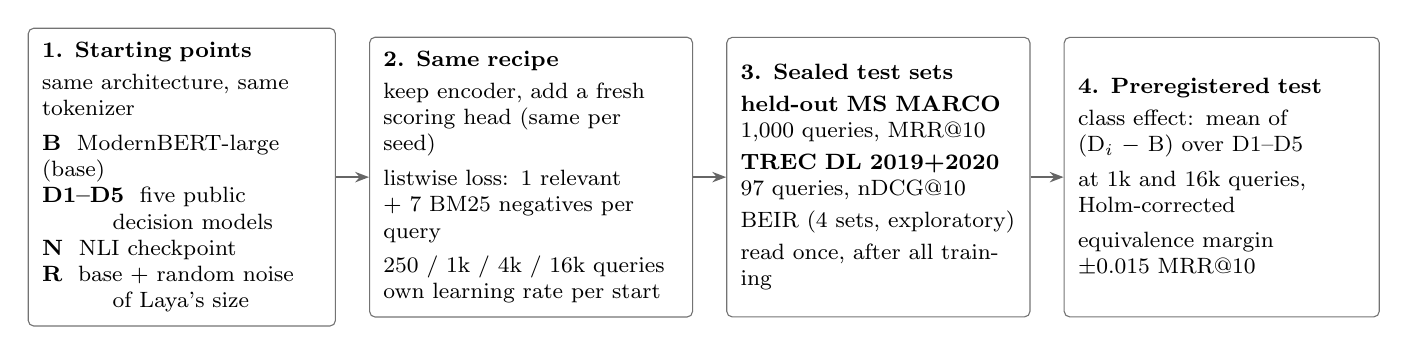
\begin{tikzpicture}[
  font=\footnotesize,
  box/.style={draw=black!55, rounded corners=2pt, align=left, inner sep=5pt, text width=#1, minimum height=3.55cm},
  head/.style={font=\footnotesize\bfseries},
  arr/.style={-{Stealth[length=5pt]}, thick, black!60},
  node distance=0.42cm
]
\node[box=3.55cm] (a) {%
  {\bfseries 1. Starting points}\\[2pt]
  same architecture, same tokenizer\\[3pt]
  \textbf{B}\ \ ModernBERT-large (base)\\
  \textbf{D1--D5}\ \ five public\\\ \ \ \ \ \ \ \ \ decision models\\
  \textbf{N}\ \ NLI checkpoint\\
  \textbf{R}\ \ base + random noise\\\ \ \ \ \ \ \ \ \ of Laya's size};
\node[box=3.75cm, right=of a] (b) {%
  {\bfseries 2. Same recipe}\\[2pt]
  keep encoder, add a fresh\\ scoring head (same per seed)\\[3pt]
  listwise loss: 1 relevant\\ + 7 BM25 negatives per query\\[3pt]
  250 / 1k / 4k / 16k queries\\
  own learning rate per start};
\node[box=3.5cm, right=of b] (c) {%
  {\bfseries 3. Sealed test sets}\\[2pt]
  \textbf{held-out MS MARCO}\\ 1{,}000 queries, MRR@10\\[2pt]
  \textbf{TREC DL 2019+2020}\\ 97 queries, nDCG@10\\[2pt]
  BEIR (4 sets, exploratory)\\[2pt]
  read once, after all training};
\node[box=3.65cm, right=of c] (d) {%
  {\bfseries 4. Preregistered test}\\[2pt]
  class effect: mean of\\ (D$_i$ $-$ B) over D1--D5\\[3pt]
  at 1k and 16k queries,\\ Holm-corrected\\[3pt]
  equivalence margin\\ $\pm$0.015 MRR@10};
\draw[arr] (a) -- (b);
\draw[arr] (b) -- (c);
\draw[arr] (c) -- (d);
\end{tikzpicture}
}
\caption{The study in four steps. Eight starting points that differ only in their weights are fine-tuned with the same recipe, each at its own selected learning rate, at four data budgets and scored on sealed test sets. The preregistered test compares the average of the five decision checkpoints with the plain encoder.}
\label{fig:design}
\end{figure*}

\subsection{Starting points}

Table~\ref{tab:arms} lists the eight arms. All use the ModernBERT-large architecture (28 layers, about 395M encoder parameters), and every encoder tensor loads into it unchanged. We took every public decision checkpoint on this backbone that we could find and that was not a copy of another. To detect copies we compare \emph{drift vectors}, the difference between a checkpoint's weights and the plain encoder's. Independently fine-tuned checkpoints have nearly orthogonal drift vectors (cosine $\leq0.04$ here), so we excluded one near-copy of Laya (cosine 0.98). Note that von is built on the NLI checkpoint (cosine 0.85). The training data in Table~\ref{tab:arms} is as stated on each model card; we could not verify it.

\begin{table}[t]
\centering
\caption{Starting points (arms). Drift is $\lVert\theta-\theta_B\rVert/\lVert\theta_B\rVert$ over encoder weights.}
\label{tab:arms}
\setlength{\tabcolsep}{3pt}
\begin{tabular}{@{}l l p{3.45cm} r@{}}
\toprule
Arm & Name & Training data (model card) & Drift \\
\midrule
B  & ModernBERT-large & masked-language pre-training only & 0 \\
D1 & Laya & undisclosed decision corpus (RL objective) & 4.94\% \\
D2 & Beveridge & operations documents and logs & 3.35\% \\
D3 & von & decision corpus incl.\ ANLI; built on N & 3.71\% \\
D4 & solvi & SQuAD 2.0, BoolQ, VitaminC & 1.40\% \\
D5 & cortex & software and security decisions & 0.68\% \\
\midrule
N  & NLI & GLUE (incl.\ QNLI) and ANLI~\cite{sileo2024tasksource} & 3.11\% \\
R  & Noise & B + Gaussian noise, per-tensor norm of D1's drift & 4.94\% \\
\bottomrule
\end{tabular}
\end{table}

Each control answers one ``maybe it's just\ldots'' question. \textbf{N} asks whether any supervised sentence-pair training gives the same head start. \textbf{R} asks whether a gain could come from moving the weights at all. For every tensor, including the embeddings, R adds Gaussian noise (seed 12345) rescaled to the norm of Laya's change to that tensor. R is therefore as far from B as the farthest decision checkpoint, but in a random direction.

Only encoder weights are transferred. Every arm gets the standard ModernBERT classification head, newly initialized: mean pooling, a dense layer with GELU and layer normalization, and a linear output. The head is initialized from the run's seed, so for a given seed all arms start from an identical head. Decision models' own heads and prompt templates are not used. The input is the usual pair format, \texttt{[CLS] query [SEP] passage [SEP]}.

\subsection{Training recipe}

All arms use the recipe in Table~\ref{tab:recipe}. Each training example is a query with its labelled relevant passage and seven negatives drawn from the BM25 top-50. The model scores all eight, and the loss is the cross-entropy of a softmax over those scores, which rewards putting the relevant passage first~\cite{gao2021rethink}. A model that guesses at random has a loss of $\ln 8=2.08$. Training queries come from the BM25-mined MS MARCO training triples, deduplicated, with every query that also appears in the TREC DL sets or the MS MARCO v1.1 validation set removed (matched after lower-casing and stripping punctuation). This leaves a pool of 25{,}906 queries. Budgets are nested: the 250-query sample is the first 250 of the 1{,}000-query sample, and so on. A different seed changes the head initialization, the sampled negatives and the data order.

\begin{table}[t]
\centering
\caption{Training recipe, identical for every arm.}
\label{tab:recipe}
\setlength{\tabcolsep}{4pt}
\begin{tabular}{@{}l p{5.1cm}@{}}
\toprule
Data & MS MARCO BM25 triples (shard 0), deduplicated, $\geq$30 distinct negatives per query \\
Budgets & 250, 1k, 4k, 16k queries (32, 125, 500, 2{,}000 steps) \\
Group / loss & 1 positive + 7 BM25 negatives; listwise softmax cross-entropy \\
Batch & 8 queries (64 pairs) per step as 2 micro-batches; one epoch \\
Optimizer & AdamW~\cite{loshchilov2019adamw}, weight decay 0.01, 10\% warm-up then linear decay, gradient clip 1.0, bf16 \\
Length & 256 tokens (train), 384 (inference, fp16) \\
Learning rate & per arm, best dev \ms{} over \{1, 2, 4, 8, 16\}$\times10^{-5}$ at 1k queries (seed 0; ties to the smaller rate); reused at all budgets \\
Seeds & 3 at 1k; 2 at 250 and 4k; at 16k, 2 for B and 1 per decision arm \\
Arms per budget & all 8 at 250 and 1k; B and D1--D5 at 4k and 16k \\
\bottomrule
\end{tabular}
\end{table}

\textbf{Why per-arm learning rates.} A starting point that has already moved away from the plain encoder may prefer a different step size. If every arm used B's best rate, a real advantage could be hidden. Tuning each rate on the test set could create a fake one. We therefore select each arm's rate on a separate development set of 500 held-out training queries, using dev scores only. The winning search run is then reused as seed 0 at 1k. We also report what happens when every arm reuses B's rate (Section~\ref{sec:specific}).

\textbf{Why these seed counts.} The compute budget was one RTX 3090 for about 12 hours. Seeds go where the preregistered test needs them most, at 1k. The 16k test relies on variation \emph{between} the five decision checkpoints rather than between seeds.

\subsection{Evaluation sets and metrics}

\textbf{Metrics.} \ms{} is the reciprocal rank of the first relevant passage, counted only if it is in the top 10 and 0 otherwise, averaged over queries. \nd{} also gives credit for partly relevant passages and rewards putting the most relevant ones first. Both range from 0 to 1. For scale: the plain encoder improves by 0.12 \ms{} between 1k and 4k training queries.

\textbf{Held-out MS MARCO (co-primary).} 1{,}000 training-split queries never used for training or development. Each has its labelled passage and the first 20 of its mined BM25 negatives, so 21 candidates in random order. Random ranking scores about 0.14 \ms{}. One run's standard error is about 0.012, and a paired difference between two arms has a standard error of about 0.008. Because the negatives come from the same mining process as the training negatives, this set measures in-distribution learning. Its labels are sparse, so some ``negatives'' may be relevant, which penalizes stronger models more~\cite{arabzadeh2022shallow}.

\textbf{TREC DL 2019 + 2020 (co-primary).} 97 queries with graded relevance judgments~\cite{craswell2020dl19,craswell2021dl20}. The official top-1{,}000 files carry no scores, so for each year we index its candidate passages with BM25 (bm25s~\cite{lu2024bm25s}, $k_1=1.2$, $b=0.75$), re-rank each query's candidates and keep the top~100. Unjudged passages count as non-relevant. BM25 order alone scores 0.480 \nd{}.

\textbf{BEIR (exploratory).} SciFact, NFCorpus and FiQA (200 random queries each) and TREC-COVID (all 50)~\cite{thakur2021beir}. These are out-of-domain tests on the BM25 top-30 from each full corpus, scored only for 4k and 16k models (seed 0).

\textbf{Reference rerankers.} For context only, we score two public MS MARCO rerankers on the same candidates: MiniLM-L6~\cite{wang2020minilm,reimers2019sbert} and bge-reranker-v2-m3~\cite{chen2024bgem3}. They are not part of any claim.

Metrics come from our own code, tested against \texttt{ir\_measures}~\cite{macavaney2022irmeasures}. fp16 and fp32 inference rank passages almost identically (Spearman 0.99998). Every test score was written to a sealed file, which one analysis script read once, after all confirmatory training had finished.

\subsection{Preregistered analysis}
\label{sec:prereg}

\textbf{What was frozen.} Tag \texttt{prereg-v1} fixed the configuration and the analysis code before any confirmatory run. The configuration covers arms, budgets, seeds, sets, equivalence margins and $\alpha$. The code covers the class effect, its intervals, Holm correction, the equivalence test, the outcome label and the stability test. Our prose design notes were kept outside the repository, and a planned registration on OSF was not made, so the tagged code and configuration are the preregistration. Before tagging, the notes had also planned a third seed at 250 and 4k, a separate learning-rate search at 250, and a secondary MS MARCO v1.1 endpoint. All three were dropped to fit the compute budget.

\textbf{Primary quantity.} For budget $b$ and decision checkpoint $i$, $\Delta_i(b)$ is D$_i$'s mean test score minus B's, with each model first averaged over its seeds. The \emph{class effect} is $\bar\Delta(b)=\frac{1}{5}\sum_{i}\Delta_i(b)$, the expected gain from picking one of these decision checkpoints instead of the plain encoder.

\textbf{Two kinds of interval.} The preregistered \emph{random-effects} interval treats the five checkpoints as a sample of decision checkpoints in general: a $t$-interval over the five $\Delta_i$ with 4 degrees of freedom. This is the claim a practitioner cares about, since their checkpoint will differ from ours. It treats B's seed mean as fixed and does not include B's own seed-to-seed variation. A secondary \emph{fixed-effects} interval holds the five checkpoints fixed and resamples queries with a paired bootstrap (10{,}000 resamples)~\cite{efron1993bootstrap,smucker2007significance}. It answers the narrower question ``are \emph{these} runs better on these queries?''. It conditions on the particular training runs, so it does not cover retraining.

\textbf{Hypothesis and outcome label.} H1 states that $\bar\Delta(1\text{k})\neq0$ and $\bar\Delta(16\text{k})\neq0$, Holm-corrected over the two budgets~\cite{holm1979}. A claim requires both co-primary sets to agree, which is an intersection--union test. The outcome label is computed on the held-out set from the random-effects results at $\alpha=0.05$:
\begin{itemize}
\item \emph{persists}: a gain at 1k and at 16k;
\item \emph{fades}: a gain at 1k, 16k equivalent to zero, and a smaller point estimate at 16k than at 1k;
\item \emph{null}: 1k equivalent to zero;
\item \emph{advantage, large budget inconclusive}: a gain at 1k with 16k unresolved;
\item \emph{inconclusive}: none of the above.
\end{itemize}
Equivalence uses two one-sided tests (TOST), i.e.\ a 90\% interval inside $\pm$0.015 \ms{} (held-out) or $\pm$0.02 \nd{} (DL, descriptive)~\cite{schuirmann1987tost,lakens2017equivalence}.

\textbf{Secondary, preregistered.}
\begin{itemize}
\item \emph{Specificity}: the decision class minus N, and minus R, at 1k, Holm-corrected over the two.
\item \emph{Stability}: a ``bad run'' is a run more than 0.05 \ms{} below its arm's median at the same budget. Bad-run counts for decision arms and B are compared with Fisher's exact test.
\item \emph{Data saving}: how many training queries B needs to match the decision class at 1k, interpolated in $\log_2$ budget.
\item \emph{Frozen probes}: whether a frozen checkpoint's probe quality predicts its fine-tuned gain (Spearman, eight arms, descriptive).
\end{itemize}

\subsection{Amendments and later changes}
\label{sec:amend}

Every change after the preregistration tag is recorded in the repository history:
\begin{enumerate}
\item \textbf{Wider learning-rate grid} (before any test score was read). The original grid \{2, 4, 8\}$\times10^{-5}$ put B's best rate on its lower edge and two decision arms on its upper edge. A grid that ends at an arm's best rate may under-tune that arm, so we widened it to \{1, 2, 4, 8, 16\}$\times10^{-5}$ for every arm. The selection rule did not change.
\item \textbf{One extra run and a failure flag} (before any test score was read). Laya's 16k run at its selected rate failed to train (Section~\ref{sec:collapse}). We added one Laya 16k run at B's rate for a labelled sensitivity analysis. We also added an objective \emph{training-failure} flag: the mean training loss over the last tenth of logged steps exceeds $0.8\ln 8=1.66$.
\item \textbf{The flag restricted to runs of at least 100 steps} (after the test scores were read). As first written, the flag caught 6 of the 16 runs at 250 queries, one of them from B (seed 0). Those runs have 32 steps, and the loss is logged as a 10-step mean, so their ``last tenth'' is a single logged value from one or two 8-query batches. That value does not track quality: one flagged von run is that arm's best at 250 queries. We therefore restricted the flag to runs of at least 100 steps.
\item \textbf{Exclusion analyses} (after the test scores were read). Every analysis that sets flagged runs aside (Sections~\ref{sec:excl} and~\ref{sec:specific}) was added after unsealing and is exploratory.
\end{enumerate}
Two code changes after the tag do not affect any confirmatory number. One sets a floor of 1/10{,}000 on bootstrap $p$-values, which could previously print as 0. The other passes segment ids correctly to the MiniLM reference, which affects only the context rows.

\section{Results}

\subsection{The preregistered answer: inconclusive}
\label{sec:primary}

Fig.~\ref{fig:curves} shows how every arm learns as data grows, and Table~\ref{tab:main} gives the numbers. Three patterns are visible before any statistics. First, at small budgets most non-base arms start well ahead. At 250 queries B reaches 0.377 \ms{}, while von, solvi and NLI exceed 0.51. Second, the arms converge: at 16k, every arm without a collapsed run averages 0.705 to 0.714 on held-out (single runs 0.704 to 0.715) and 0.62 to 0.64 on DL. Third, a few runs sit far below their arm's curve. These are the collapsed runs (hollow markers), discussed in Section~\ref{sec:collapse}.

\begin{figure*}[t]
\centering
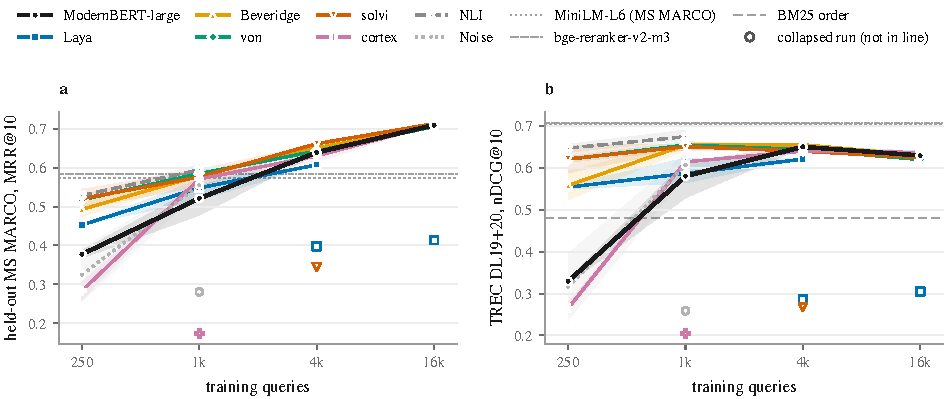
\includegraphics[width=\textwidth]{f1_learning_curves.pdf}
\caption{Learning curves. (a) Held-out MS MARCO, \ms{}. (b) TREC DL 2019+2020, \nd{}. Lines connect seed means of runs that did not collapse, and shaded bands span the seeds. Hollow markers are collapsed runs, plotted separately (Table~\ref{tab:main} includes them in its means, so some values differ). Horizontal lines are context: two public rerankers and, on DL, BM25 order. The 16k models outscore the public rerankers on (a), which shares the training distribution, but not on (b).}
\label{fig:curves}
\end{figure*}

\begin{table*}[t]
\centering
\caption{Mean test score over seeds for every arm and budget, all runs included as preregistered. \fl{}: the mean includes a collapsed run. Seed counts are in Table~\ref{tab:recipe}. The class effect is the mean of D1--D5 minus B, with its random-effects 95\% interval.}
\label{tab:main}
\setlength{\tabcolsep}{5pt}
\begin{tabular}{@{}l cccc c cccc@{}}
\toprule
& \multicolumn{4}{c}{Held-out MS MARCO (\ms{})} && \multicolumn{4}{c}{TREC DL 19+20 (\nd{})} \\
\cmidrule{2-5}\cmidrule{7-10}
Arm & 250 & 1k & 4k & 16k && 250 & 1k & 4k & 16k \\
\midrule
B (ModernBERT-large) & 0.377 & 0.521 & 0.639 & 0.710 && 0.329 & 0.580 & 0.650 & 0.629 \\
D1 Laya & 0.453 & 0.548 & 0.503\fl & 0.414\fl && 0.554 & 0.587 & 0.454\fl & 0.305\fl \\
D2 Beveridge & 0.493 & 0.580 & 0.651 & 0.705 && 0.558 & 0.655 & 0.655 & 0.630 \\
D3 von & 0.517 & 0.585 & 0.643 & 0.706 && 0.620 & 0.655 & 0.644 & 0.620 \\
D4 solvi & 0.521 & 0.576 & 0.503\fl & 0.714 && 0.621 & 0.651 & 0.454\fl & 0.624 \\
D5 cortex & 0.283 & 0.439\fl & 0.631 & 0.711 && 0.265 & 0.478\fl & 0.640 & 0.637 \\
N (NLI) & 0.529 & 0.595 & -- & -- && 0.647 & 0.674 & -- & -- \\
R (Noise) & 0.324 & 0.464\fl & -- & -- && 0.316 & 0.491\fl & -- & -- \\
\midrule
Class effect & \p0.076 & \p0.025 & \m0.053 & \m0.060 && \p0.194 & \p0.024 & \m0.081 & \m0.066 \\
95\% interval & {\scriptsize[\m.047, .199]} & {\scriptsize[\m.052, .101]} & {\scriptsize[\m.148, .042]} & {\scriptsize[\m.224, .104]} && {\scriptsize[.011, .378]} & {\scriptsize[\m.071, .120]} & {\scriptsize[\m.212, .050]} & {\scriptsize[\m.245, .113]} \\
\midrule
\multicolumn{10}{@{}l}{\textit{Context} (held-out / DL): random order 0.14 / --- \quad BM25 order --- / 0.480 \quad MiniLM-L6 0.573 / 0.704 \quad bge-reranker-v2-m3 0.584 / 0.707} \\
\bottomrule
\end{tabular}
\end{table*}

The preregistered test asks about the class effect at 1k and 16k. At 1k the five decision checkpoints are on average $+0.025$ \ms{} ahead on held-out (95\% CI $-0.052$ to $+0.101$) and $+0.024$ \nd{} on DL ($-0.071$ to $+0.120$). At 16k they are $-0.060$ ($-0.224$ to $+0.104$) and $-0.066$ ($-0.245$ to $+0.113$). Both Holm-adjusted $p$-values are 0.74, and neither budget passes the equivalence test. The preregistered label is therefore \textbf{inconclusive}: the data cannot rule out a gain, a loss or no difference for decision checkpoints in general.

The fixed-effects analysis asks only about these particular runs. It gives $+0.025$ ($+0.012$ to $+0.037$) at 1k and $-0.060$ ($-0.071$ to $-0.049$) at 16k. The 16k loss comes from one run, Laya's, at $-0.296$. The other four checkpoints are within 0.005 of B (Fig.~\ref{fig:forest}). Without Laya, the 16k fixed-effects estimate on held-out would be $-0.001$. The preregistered data-saving summary agrees that the effect is modest: B needs about 1{,}330 training queries to match what the decision class reaches with 1{,}000, i.e.\ 33\% more data. Dropping solvi, the checkpoint with the most question--passage supervision (a robustness check from our design notes), makes the 1k class effect smaller ($+0.017$, 95\% CI $-0.092$ to $+0.125$).

\begin{figure*}[t]
\centering
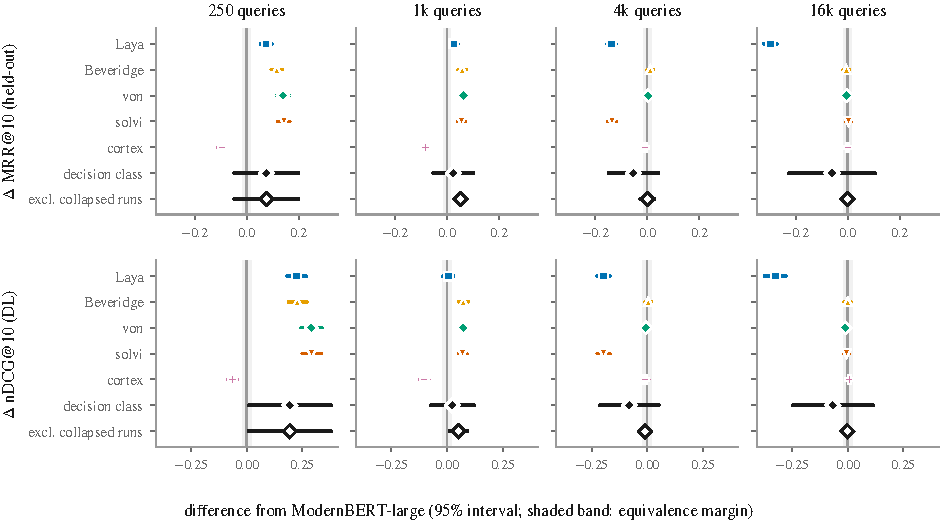
\includegraphics[width=\textwidth]{f2_forest.pdf}
\caption{Difference from the plain encoder, per checkpoint and for the class, at each budget. Per-checkpoint intervals resample queries only (fixed-effects). The ``decision class'' interval is the preregistered random-effects interval, which also reflects disagreement between checkpoints and is therefore much wider. ``Excl.\ collapsed runs'' is the exploratory analysis of Section~\ref{sec:excl}; at 250 queries no run is excluded, so the two rows coincide. Shaded band: equivalence margin.}
\label{fig:forest}
\end{figure*}

\subsection{Why: some runs collapse}
\label{sec:collapse}

The class intervals are wide because of a few runs, not because every checkpoint behaves slightly differently. Fig.~\ref{fig:loss} shows the most extreme case. At 16k queries every arm's training loss falls smoothly from about 2 to about 0.7, except Laya's at its selected rate of $1.6\times10^{-4}$. Its loss first falls to about 1.25, then climbs back to about 2.0 by step 380, and settles near 1.7 for the rest of training. The resulting model scores 0.414 \ms{}, far below the other 16k models (0.704 to 0.715). The same checkpoint at B's rate of $2\times10^{-5}$ trains normally.

\begin{figure}[t]
\centering
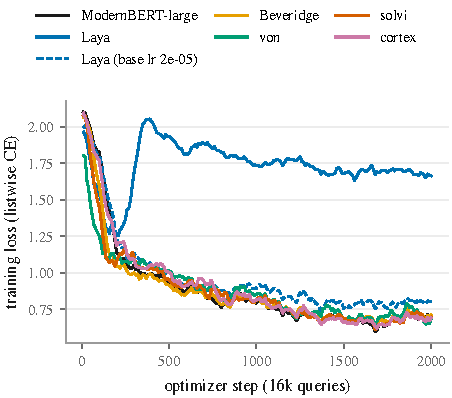
\includegraphics[width=\columnwidth]{fa2_loss.pdf}
\caption{Training loss at 16k queries (moving average). Laya at its selected learning rate ($1.6\times10^{-4}$) improves briefly, climbs back towards the random-guess loss of $\ln 8=2.08$, and stays near 1.7. At the plain encoder's rate (dashed) it trains normally.}
\label{fig:loss}
\end{figure}

Table~\ref{tab:failures} lists every run caught by the training-failure flag. Five of the 59 runs in the preregistered analysis collapsed: four from decision checkpoints and one from the noise control. Their test scores, 0.17 to 0.41 \ms{}, are well below the 0.54 to 0.66 of the same arm's other runs at that budget. None came from B, N, Beveridge or von. All five ran above B's rate, two of them at 1k, the very budget at which the rates were chosen. A rate that worked on one seed can therefore fail on another seed at the same budget, as well as over the longer runs at 4k and 16k.

\begin{table}[t]
\centering
\caption{Runs flagged as training failures (mean loss over the last tenth of steps $>1.66$, runs of $\geq$100 steps). Random guessing gives 2.08; Laya at 16k sits just above the threshold.}
\label{tab:failures}
\setlength{\tabcolsep}{4pt}
\begin{tabular}{@{}l r r r c c@{}}
\toprule
Arm & Budget & LR & Seed & Final loss & Held-out \\
\midrule
D1 Laya & 16k & $1.6\times10^{-4}$ & 0 & 1.67 & 0.414 \\
D1 Laya & 4k & $1.6\times10^{-4}$ & 1 & 1.71 & 0.398 \\
D4 solvi & 4k & $4\times10^{-5}$ & 1 & 1.78 & 0.345 \\
D5 cortex & 1k & $4\times10^{-5}$ & 2 & 2.09 & 0.173 \\
R Noise & 1k & $4\times10^{-5}$ & 2 & 1.98 & 0.280 \\
\bottomrule
\end{tabular}
\end{table}

\textbf{Checkpoint or learning rate?} The learning-rate search (Fig.~\ref{fig:lrgrid}) shows two kinds of arm. B, cortex and Noise peak at 2 to $4\times10^{-5}$; cortex and Noise fall sharply at $8\times10^{-5}$, and B at $1.6\times10^{-4}$, where it scores only 0.354 dev \ms{}. The other decision arms and N stay flat or keep improving up to $1.6\times10^{-4}$, and Laya's best rate is the largest we tried. B never trained above $2\times10^{-5}$ in a confirmatory run. These data therefore cannot separate ``these checkpoints are fragile'' from ``these learning rates are fragile''. What they do show is that choosing the rate on a single short run can pick one that fails on other seeds or longer runs.

\begin{figure}[t]
\centering
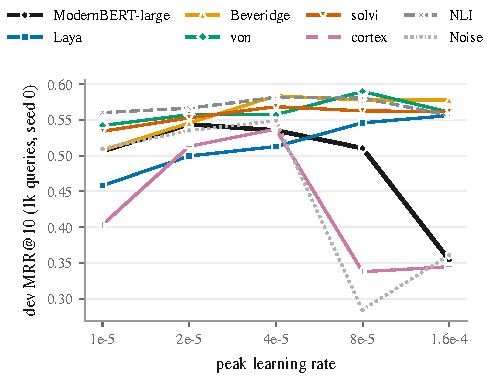
\includegraphics[width=\columnwidth]{fa1_lr_grid.pdf}
\caption{Learning-rate search (dev \ms{}, 1k queries, seed 0). The plain encoder prefers $2\times10^{-5}$ and fails at $1.6\times10^{-4}$. Most supervised checkpoints tolerate much larger rates. Laya's best is the edge of the grid.}
\label{fig:lrgrid}
\end{figure}

The preregistered stability test does not separate decision arms from B: 3 of 40 decision runs versus 1 of 9 base runs are ``bad runs'' (Fisher's exact $p=0.57$). The training-failure flag gives 4 of 40 versus 0 of 9 ($p=1.0$). The bad-run rule compares each run with its own arm's median, so it misses collapses in arms with a single seed (Laya at 16k). B's one ``bad run'' (seed 1 at 1k, 0.478 \ms{}) is ordinary seed variance, not a collapse: its loss fell normally. Our design notes also listed a cruder measure, runs that score below BM25 on DL. These are 2 of 9 for B (both at 250 queries), 6 of 40 for decision arms, 0 of 5 for N and 3 of 5 for R.

\subsection{Without the collapses: a small head start that fades}
\label{sec:excl}

Collapses are a real cost of these starting points, and they stay in the preregistered result. A practitioner who notices a failed run will usually retrain it, though, so it is worth asking what decision checkpoints give when training works. Table~\ref{tab:sens} answers this with exploratory analyses that drop the flagged runs and repeat the same computations. All of these analyses were chosen after the test scores were read.

\begin{table}[t]
\centering
\caption{Class effect (D1--D5 minus B) at 1k unless stated; random-effects 95\% interval. Rows below the preregistered ones are exploratory, except the last, which is the pre-unsealing sensitivity run of amendment 2.}
\label{tab:sens}
\resizebox{\columnwidth}{!}{%
\begin{tabular}{@{}l l c c@{}}
\toprule
Analysis & Budget & Held-out \ms{} & DL \nd{} \\
\midrule
\multirow{2}{*}{Preregistered} & 1k & \p0.025 [\m0.052, \p0.101] & \p0.024 [\m0.071, \p0.120] \\
& 16k & \m0.060 [\m0.224, \p0.104] & \m0.066 [\m0.245, \p0.113] \\
\midrule
\multirow{3}{*}{Excl.\ collapsed runs} & 1k & \p\textbf{0.051} [\p0.033, \p0.069] & \p\textbf{0.052} [\p0.014, \p0.090] \\
& 4k & \m0.000 [\m0.027, \p0.026] & \m0.010 [\m0.025, \p0.005] \\
& 16k$^{a}$ & \m0.001 [\m0.007, \p0.005] & \m0.002 [\m0.013, \p0.010] \\
\midrule
\quad also excl.\ B's weakest seed & 1k & \p0.029 [\p0.012, \p0.047] & \p0.026 [\m0.012, \p0.064] \\
\quad seed 0 only (search runs) & 1k & \p0.028 [\p0.014, \p0.041] & \p0.010 [\m0.030, \p0.051] \\
\quad seeds 1--2 only & 1k & \p0.063 [\p0.040, \p0.086] & \p0.072 [\p0.035, \p0.110] \\
\midrule
Laya at B's rate & 16k & \m0.014 [\m0.050, \p0.022] & \p0.004 [\m0.014, \p0.021] \\
\bottomrule
\multicolumn{4}{@{}l}{\footnotesize $^{a}$Four checkpoints: Laya's only 16k run collapsed.}
\end{tabular}}
\end{table}

With the collapsed runs set aside, decision checkpoints lead at 1k by $+0.051$ \ms{} on held-out and $+0.052$ \nd{} on DL. All five checkpoints are individually ahead on held-out ($+0.027$ to $+0.064$), and the class is ahead in each of the three seeds ($+0.028$, $+0.090$, $+0.035$). At 4k the estimate is zero, though its interval is too wide to show equivalence. At 16k it is $-0.001$, with a 90\% interval of $[-0.006,+0.004]$, well inside the $\pm$0.015 margin (DL: $[-0.010,+0.007]$, inside $\pm$0.02). Applying the preregistered rule to these numbers gives \textbf{fades}. The 1k advantage holds on both sets (Holm-adjusted intersection--union $p=0.04$), and 16k is equivalent to zero.

How large is the head start? Two things make the $+0.05$ estimate an upper end. First, B's three seeds at 1k vary widely (0.553, 0.478, 0.533), and the random-effects interval does not include this uncertainty. Also dropping B's weakest seed gives $+0.029$ on held-out but only $+0.026$ on DL, whose interval covers zero, so the two sets no longer agree. Second, the seed-0 runs double as the learning-rate search, so they could be lucky. Here the opposite holds: the seed-0 effect ($+0.028$) is smaller than the effect on seeds 1 and 2 ($+0.063$). Our best summary is a head start of about $+0.03$ to $+0.05$ \ms{} at 1k that is gone by 16k.

Laya at 16k is the case most sensitive to how a collapse is handled. Swapping in its run at B's rate, instead of dropping it, gives a class effect of $-0.014$ ($-0.050$ to $+0.022$) on held-out. That interval covers zero but is too wide to show equivalence, so under this handling 16k is unresolved. That Laya run trains normally but ends below B on held-out (0.645 vs.\ 0.710) and above it on DL (0.656 vs.\ 0.629).

At 250 queries, which the preregistration treats as descriptive, the picture is larger but uneven. Four checkpoints are 0.08 to 0.14 \ms{} ahead of B, while cortex is 0.09 behind (Fig.~\ref{fig:forest}). Cortex has the smallest drift from B (0.68\%), and at 250 queries it behaves like an unlucky plain encoder, not like a pre-trained ranker.

\subsection{Is the head start about decisions?}
\label{sec:specific}

The preregistered NLI contrast says \textbf{no}; the noise contrast agrees only in the exploratory analysis without collapsed runs. Table~\ref{tab:spec} and Fig.~\ref{fig:spec} compare the decision class with both controls on identical queries.

\begin{table*}[t]
\centering
\caption{Contrasts at 1k (query-bootstrap 95\% intervals, which do not cover retraining). Left: all runs; the decision$-$NLI and decision$-$Noise rows are the preregistered specificity tests (Holm $p<0.001$ for both). Right: the same contrasts with collapsed runs excluded, treating controls and decision arms alike (exploratory).}
\label{tab:spec}
\setlength{\tabcolsep}{5pt}
\begin{tabular}{@{}l cc c cc@{}}
\toprule
& \multicolumn{2}{c}{All runs (preregistered)} && \multicolumn{2}{c}{Collapsed runs excluded (exploratory)} \\
\cmidrule{2-3}\cmidrule{5-6}
Contrast at 1k & Held-out \ms{} & DL \nd{} && Held-out \ms{} & DL \nd{} \\
\midrule
Decision class $-$ B & \p0.025 [\p0.012, \p0.037] & \p0.024 [\p0.006, \p0.044] && \p0.051 [\p0.039, \p0.064] & \p0.052 [\p0.033, \p0.071] \\
NLI $-$ B & \p0.074 [\p0.058, \p0.090] & \p0.094 [\p0.070, \p0.119] && \p0.074 [\p0.058, \p0.090] & \p0.094 [\p0.070, \p0.119] \\
Noise $-$ B & \m0.057 [\m0.071, \m0.044] & \m0.090 [\m0.110, \m0.069] && \p0.034 [\p0.021, \p0.048] & \p0.026 [\p0.010, \p0.044] \\
\midrule
Decision class $-$ NLI & \m0.049 [\m0.059, \m0.039] & \m0.070 [\m0.085, \m0.055] && \m0.023 [\m0.033, \m0.012] & \m0.042 [\m0.058, \m0.028] \\
Decision class $-$ Noise & \p0.082 [\p0.070, \p0.094] & \p0.114 [\p0.096, \p0.133] && \p0.017 [\p0.005, \p0.029] & \p0.025 [\p0.010, \p0.041] \\
\bottomrule
\end{tabular}
\end{table*}

\begin{figure*}[t]
\centering
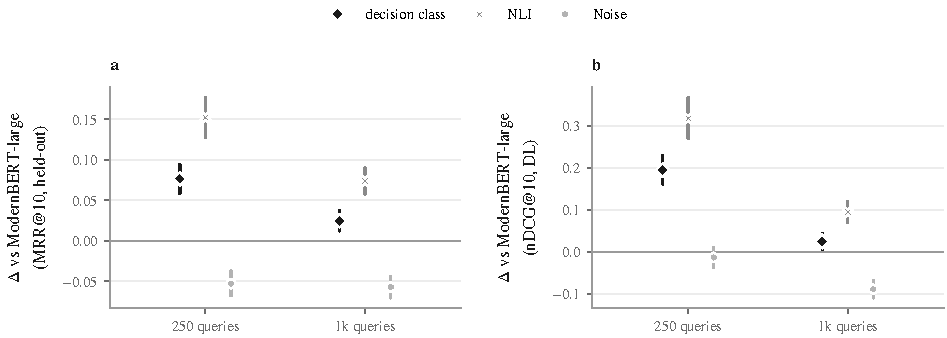
\includegraphics[width=0.82\textwidth]{f3_specificity.pdf}
\caption{Difference from the plain encoder for the decision class and the two controls (all runs, as preregistered; query-bootstrap 95\% intervals). The Noise arm's position at 1k is driven by its one collapsed run; see Table~\ref{tab:spec} for the comparison without collapsed runs.}
\label{fig:spec}
\end{figure*}

\textbf{NLI is the stronger starting point.} With all runs, the decision class trails NLI by 0.049 \ms{} and 0.070 \nd{} at 1k, and by 0.076 and 0.123 at 250. With collapsed runs excluded, it still trails by 0.023 and 0.042. NLI never collapsed, but it was trained only up to 1k, so its stability at larger budgets is untested. This is one NLI checkpoint, so the claim is about this checkpoint, not NLI training in general. Von, which is decision training on top of this same NLI checkpoint, lands slightly below it at 1k ($-0.010$ \ms{}, $-0.020$ \nd{}). Adding decision training on top of NLI did not help.

\textbf{Even random noise helps, when it trains.} With all runs, the preregistered contrast says the decision class beats noise by a wide margin. That margin comes from the noise arm's collapsed run. Treating the controls like the decision arms and excluding that run, noise itself is $+0.034$ \ms{} ahead of B, and the decision class leads noise by only $+0.017$ ($+0.005$ to $+0.029$). So a random move of the same size as Laya's change, followed by fine-tuning at a higher rate, recovers about two-thirds of the decision head start. This rests on one noise draw and two surviving seeds. We do not know why it happens, but it means most of the head start cannot be credited to what decision training taught.

\textbf{The rate is part of the effect.} When every arm reuses B's rate ($2\times10^{-5}$, one seed), the 1k class effect is $-0.001$ \ms{} ($-0.039$ to $+0.038$) and $+0.004$ \nd{} ($-0.045$ to $+0.053$). For comparison, the matching seed-0 effect at tuned rates is $+0.028$ and $+0.010$. With one seed and intervals of $\pm$0.04, we detect no decision head start at B's rate. NLI at B's rate still leads B by 0.029 \ms{} (one seed).

\subsection{What the frozen encoder already knows}

Does a checkpoint's head start show up before any reranker training? We freeze each encoder and fit a logistic-regression probe~\cite{alain2016probes} on its mean-pooled features from every fourth layer. The probe uses 8{,}000 standardized query--passage pairs (1k queries in the 1+7 format) and ranks the development set. Fig.~\ref{fig:probes}(a) shows probe quality by layer. All arms are equal at the embedding layer. From the middle layers on, NLI, solvi and von carry the most relevance signal (best layer 0.42 to 0.44 \ms{}, against 0.36 for B), while cortex and Noise are no better than B. Fig.~\ref{fig:probes}(b) shows the preregistered comparison. Across all eight arms, the frozen probe's advantage over B predicts the fine-tuned advantage at 1k (Spearman $\rho=0.90$, exact permutation $p=0.005$). Among the five decision checkpoints alone, $\rho=0.70$ ($p=0.23$). These fine-tuned gains include collapsed runs, which pull cortex and Noise down; excluding them gives $\rho=0.76$ ($p=0.04$). Frozen features may therefore be a cheap screen for which starting points are worth fine-tuning, in line with earlier work on choosing intermediate tasks~\cite{poth2021pretrain,kornblith2019transfer}.

\begin{figure*}[t]
\centering
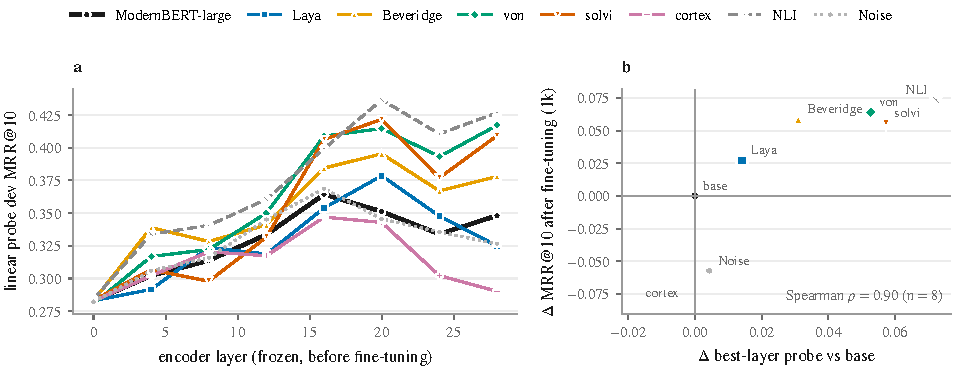
\includegraphics[width=\textwidth]{f4_probes.pdf}
\caption{(a) Frozen-feature linear probes: dev \ms{} by encoder layer, before any reranker training. (b) Best-layer probe advantage over B against fine-tuned advantage at 1k (held-out, all runs, as preregistered; cortex and Noise include their collapsed seeds).}
\label{fig:probes}
\end{figure*}

\subsection{Where fine-tuning ends up}

If the head start vanishes at 16k, do the fine-tuned models become the same model? We measure, layer by layer, the relative $L_2$ distance between each fine-tuned arm and the fine-tuned B, divided by the same distance before fine-tuning (Fig.~\ref{fig:conv}). A ratio of 1 means fine-tuning left the starting gap unchanged. At 1k the layer-averaged ratio is 1.00 to 1.20 for every arm. At 16k it is about 1.1 for most arms and larger for solvi and cortex, mostly because they start so close to B that small absolute changes produce large ratios. (Laya's 16k curve is its collapsed run.) The models do not converge to a common point, yet those that trained normally rank equally well. This is consistent with the view that fine-tuned models stay near their starting point~\cite{neyshabur2020transferred}: the head start fades because extra data teaches every model the task, not because the models become the same.

\begin{figure*}[t]
\centering
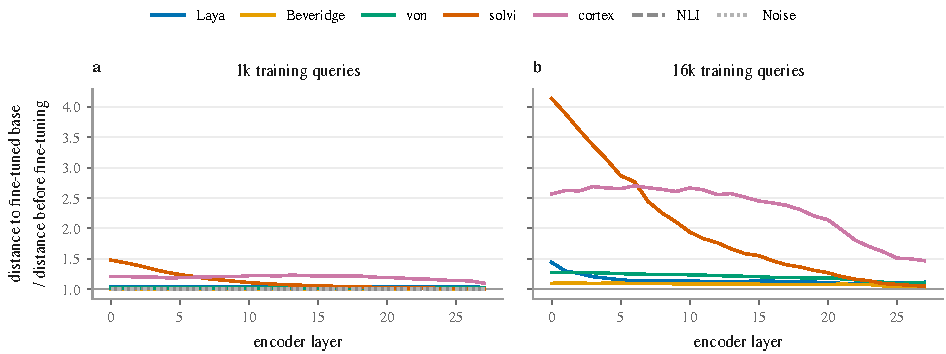
\includegraphics[width=\textwidth]{f5_convergence.pdf}
\caption{Per-layer distance between each fine-tuned arm and fine-tuned B, divided by the same distance before fine-tuning (seed 0). Values above 1: fine-tuning moved the models further apart. (a) 1k queries. (b) 16k queries (only B and D1--D5 were trained at 16k; Laya's curve is its collapsed run).}
\label{fig:conv}
\end{figure*}

\subsection{Out-of-domain transfer (exploratory)}

Table~\ref{tab:beir} reports zero-shot \nd{} on four BEIR sets for the 4k and 16k models (seed 0). There is no consistent advantage for decision checkpoints. Solvi and von are best on SciFact at 4k and Beveridge on FiQA, while collapsed Laya at 16k is worst on all four. In these single-seed results, more MS MARCO data does not reliably help transfer: B drops from 0.590 to 0.512 on SciFact between 4k and 16k. On SciFact every model we trained matches or falls below BM25 alone (0.690), while bge-reranker-v2-m3, trained on far more and more varied data, reaches 0.751. Rerankers fine-tuned on a few thousand MS MARCO queries learn MS MARCO first, and that does not automatically carry over to other domains. On DL, too, \nd{} is slightly lower at 16k than at 4k for most arms (B: 0.650 to 0.629) while held-out \ms{} keeps rising, though with 97 queries this dip is within noise.

\begin{table}[t]
\centering
\caption{Zero-shot BEIR \nd{} on the BM25 top-30 (seed 0; exploratory). \fl{}: collapsed run.}
\label{tab:beir}
\setlength{\tabcolsep}{3.5pt}
\begin{tabular}{@{}l c cccc@{}}
\toprule
Arm & Budget & SciFact & NFCorpus & FiQA & TREC-COVID \\
\midrule
\multirow{2}{*}{B} & 4k & 0.590 & 0.319 & 0.337 & 0.729 \\
 & 16k & 0.512 & 0.321 & 0.317 & 0.684 \\
\multirow{2}{*}{D1 Laya} & 4k & 0.564 & 0.293 & 0.282 & 0.701 \\
 & 16k & 0.358\fl & 0.223\fl & 0.223\fl & 0.621\fl \\
\multirow{2}{*}{D2 Beveridge} & 4k & 0.504 & 0.327 & 0.383 & 0.737 \\
 & 16k & 0.608 & 0.331 & 0.325 & 0.674 \\
\multirow{2}{*}{D3 von} & 4k & 0.660 & 0.336 & 0.343 & 0.727 \\
 & 16k & 0.590 & 0.299 & 0.279 & 0.674 \\
\multirow{2}{*}{D4 solvi} & 4k & 0.690 & 0.342 & 0.351 & 0.705 \\
 & 16k & 0.573 & 0.330 & 0.341 & 0.692 \\
\multirow{2}{*}{D5 cortex} & 4k & 0.540 & 0.310 & 0.341 & 0.729 \\
 & 16k & 0.518 & 0.318 & 0.315 & 0.692 \\
\midrule
BM25 order & -- & 0.690 & 0.332 & 0.268 & 0.609 \\
MiniLM-L6 & -- & 0.687 & 0.356 & 0.341 & 0.692 \\
bge-reranker-v2-m3 & -- & 0.751 & 0.348 & 0.392 & 0.740 \\
\bottomrule
\end{tabular}
\end{table}

\subsection{Robustness and cost}

\textbf{Pooling.} With the \texttt{[CLS]} vector instead of mean pooling (1k, seed 0, held-out), B scores 0.557 (mean pooling: 0.553) and solvi 0.622 (0.595). Laya at $1.6\times10^{-4}$ collapses with \texttt{[CLS]} pooling (0.334), one more sign of instability at that rate.

\textbf{Compute.} The 95 training runs (40 for the learning-rate search, 52 confirmatory including the one sensitivity run, and 3 for pooling) took 4.1 GPU-hours on one RTX 3090 (350 W), at 129 training pairs per second and at most 16.6~GB of memory. Scoring took a further 1.4 GPU-hours. Including pilot experiments, the project used about 9.6 GPU-hours. Training can be interrupted and resumed exactly; the largest difference in scores after a resume was $7\times10^{-5}$.

\section{Discussion}

\textbf{What should a practitioner do?} With a few thousand labelled queries or more, the starting point did not matter here, and the plain encoder at its own rate trained reliably. With fewer, a supervised checkpoint on the same backbone is worth trying. Our data point to the NLI checkpoint first: it gave the largest head start at 250 and 1k queries and did not collapse there. Whichever checkpoint is used, three habits matter more than the choice of checkpoint. Search its learning rate, since the head start depends on it. Check that rate on more than one seed, since a rate chosen on one run failed on others. And watch the training loss, since a collapsed run looks like an ordinary one until it is evaluated. A frozen-feature probe, which costs minutes, ranked our starting points much as fine-tuning did and could screen candidates before any fine-tuning.

\textbf{Why are some runs fragile?} We can only offer a hypothesis. Supervised checkpoints already contain a useful pair-scoring function, so a larger step size exploits it faster and wins on a short development run. The same step size, on another seed or over a longer run, can push the model out of that useful region before the new head has learned to use it. Laya's loss curve, which first falls quickly and then climbs back, fits this picture. Choosing a rate on one seed at one budget and reusing it elsewhere is common and economical, and it is exactly what exposed this risk. Preferring the largest rate that is stable across seeds might avoid most collapses, but we did not test this.

\textbf{Why does the head start fade, and why does noise help?} Every arm that trained normally reaches the same held-out score at 16k, yet the models stay apart in weight space. The natural reading is that NLI or decision training gives a better first guess at relevance. That guess matters when the reranker has seen few examples and is overwritten once it has seen enough, matching the finding that intermediate-task gains are largest when target data is small~\cite{phang2018stilts,pruksachatkun2020intermediate,mokrii2021transfer}. The noise result complicates this reading. Part of the head start may come from leaving the plain encoder's exact weights and training at a higher rate, not from anything a checkpoint learned. One noise draw is too little to settle this, and it is the most useful follow-up experiment we can suggest.

\subsection{Limitations}

\textbf{One backbone, five checkpoints.} ModernBERT-large is the only backbone with five independent public decision checkpoints, so our claims are scoped to it. With five checkpoints, the random-effects test has four degrees of freedom. That test generalizes beyond our checkpoints but has little power, which is part of why the preregistered answer is inconclusive. N and R are single checkpoints, and each was trained only up to 1k.

\textbf{Checkpoint provenance.} The decision checkpoints are community releases whose training data we cannot verify. One (von) is built on the NLI checkpoint, which blurs the line between decision and NLI training for that arm.

\textbf{Exploratory conclusions.} The ``head start that fades'' result depends on excluding collapsed runs, and that analysis and the final form of the flag were fixed after the test scores were read. The size of the head start also depends on B's seed-to-seed variation, which our intervals do not include.

\textbf{Learning rate.} Laya's selected rate is the largest in the grid, so it may be under-tuned at 1k. Its 16k collapse at that rate suggests that searching higher would not have helped at larger budgets. B was never trained above its own best rate in a confirmatory run, so fragility cannot be attributed to the checkpoints rather than the rates.

\textbf{Scale and seeds.} 16k queries is small next to production training sets, and decision runs at 16k have one seed each. Our claim is about data efficiency in the low-to-moderate regime, not about the best achievable reranker.

\textbf{Evaluation.} The held-out set shares the training distribution and has sparse labels. It measures learning well but favours models fitted to MS MARCO, which is why our 16k models outscore the public rerankers there but not on DL (Table~\ref{tab:main}). On DL we count unjudged passages as non-relevant and do not report how many of them reach the top 10. The preregistration is a git tag in our own repository, not an entry in an independent registry.

\section{Conclusion}

We asked whether a public decision checkpoint is a better place to start training a cross-encoder reranker than its plain encoder. Under a preregistered, multi-seed comparison with per-arm learning rates, the answer is inconclusive, because some runs from these checkpoints collapse. When training works, decision checkpoints give a head start of about 0.03 to 0.05 \ms{} at 1{,}000 training queries, gone by 16{,}000. Most of that head start is not specific to decision training. An NLI checkpoint gives more, and in an exploratory analysis even a random perturbation, trained at a higher rate, recovers much of it. Two practical lessons concern method more than decision models. A starting point should be compared at its own learning rate, on several seeds, with failed runs detected rather than averaged in. And a cheap frozen probe already tells much of the story.

\section*{Reproducibility}

The repository contains the frozen configuration and the preregistration tags (\texttt{prereg-v1}; \texttt{prereg-v1.1} records amendment 1). It also has all training and analysis code with unit tests (metrics are checked against \texttt{ir\_measures}), every run's configuration, status and training log, per-query test scores, and the scripts that regenerate every table and figure. Runs are deterministic given the seed, up to GPU non-determinism. Checkpoint revisions are listed in Table~\ref{tab:revisions}. Software: Python 3.12, PyTorch 2.15, Transformers 5.24, CUDA 13.2.

\begin{table*}[t]
\centering
\caption{Hugging Face checkpoint revisions used.}
\label{tab:revisions}
\footnotesize
\begin{tabular}{@{}l l l@{}}
\toprule
Arm & Repository & Revision \\
\midrule
B & answerdotai/ModernBERT-large & 45bb4654a4d5aaff24dd11d4781fa46d39bf8c13 \\
D1 & convaiinnovations/laya (subfolder laya-en) & fd4f9dbcf4fde222fd43174bdd4c3b08b789e4e1 \\
D2 & sathiskumarjothi0/Beveridge-Large-C & 7cb0d24cce8572b8803a738c083b2419cdc40a8a \\
D3 & mohdvasim/von & 8d072bdeb53523a1892d1382406e21c21c56fbda \\
D4 & solvi-ai/solvi-large & cd992673d838761c669611e2f59ba9661d7b1a15 \\
D5 & mukti-sys/cortex-1-large & 3fe2c0b1f997a82339dd13598759abee96495b6d \\
N & tasksource/ModernBERT-large-nli & ca476cb923a8637073d4ceb0f19f7fc236e260d4 \\
reference & cross-encoder/ms-marco-MiniLM-L6-v2 & 233902d25c440f23af6f7d6e94d2946bac0bee0a \\
reference & BAAI/bge-reranker-v2-m3 & 953dc6f6f85a1b2dbfca4c34a2796e7dde08d41e \\
\bottomrule
\end{tabular}
\end{table*}

\section*{Acknowledgment}

An AI assistant (Claude, Anthropic) was used to help write and test code and to draft and edit parts of this manuscript. The authors designed the study, checked every number against the released results, and take full responsibility for the content.

\bibliographystyle{IEEEtran}
\bibliography{../refs}

\end{document}
